\chapter{Implementation}

Differential GPS was evaluated as a suitable method to enhance the GPS position accuracy to the required level of 1 meter RMS.
This chapter documents the process of implementing it as a proof of concept.
Although this project is not planned to be used by ARIS in this years competition, the system is designed to work with the current hardware of project TELL.
Section \ref{sec:tell_infrastructure} shows what is already implemented in project TELL.
How DGPS can be integrated into this infrastructure is explained from section \ref{sec:system_overview} onward.


\section{TELL Organization and Infrastructure}\label{sec:tell_infrastructure}

At the time of writing, the competition rocket of project TELL is being made ready to ship to the U.S. for the 2018 Spaceport America Cup.
The whole project is divided into the 7 subteams: Simulations, Structures, Propulsion, Avionics, Control, and Recovery.
This bachelor thesis is a project of the Avionics subteam.
The Avionics subteam is responsible for the sensor data acquisition, which is used by the control and for logging.
It is also responsible for a telemetry link to a ground station that transmits the most important metrics to monitor the flight performance and recover the rocket.
Apart from the rockets which are also called TELL, the hardware consists of a ground station with laptop, telemetry link, and GPS reference station.

\subsection{The Rocket}

TELL is the vehicle that shall propel the 4 kg payload to the target apogee of 10'000 feet (3048 meters) at the competition.
In figure \ref{fig:tell_1} it is shown in the wind tunnel test.
It has a length of 2.42 meters, weights 24 kg at liftoff, and is propelled by a solid motor with an average thrust of 2245 N.
With those parameters, the rocket is designed to overshoot the target apogee.
Air brakes driven by a control loop are used to correct the apogee.

\begin{figure}[ht]
 \centering
 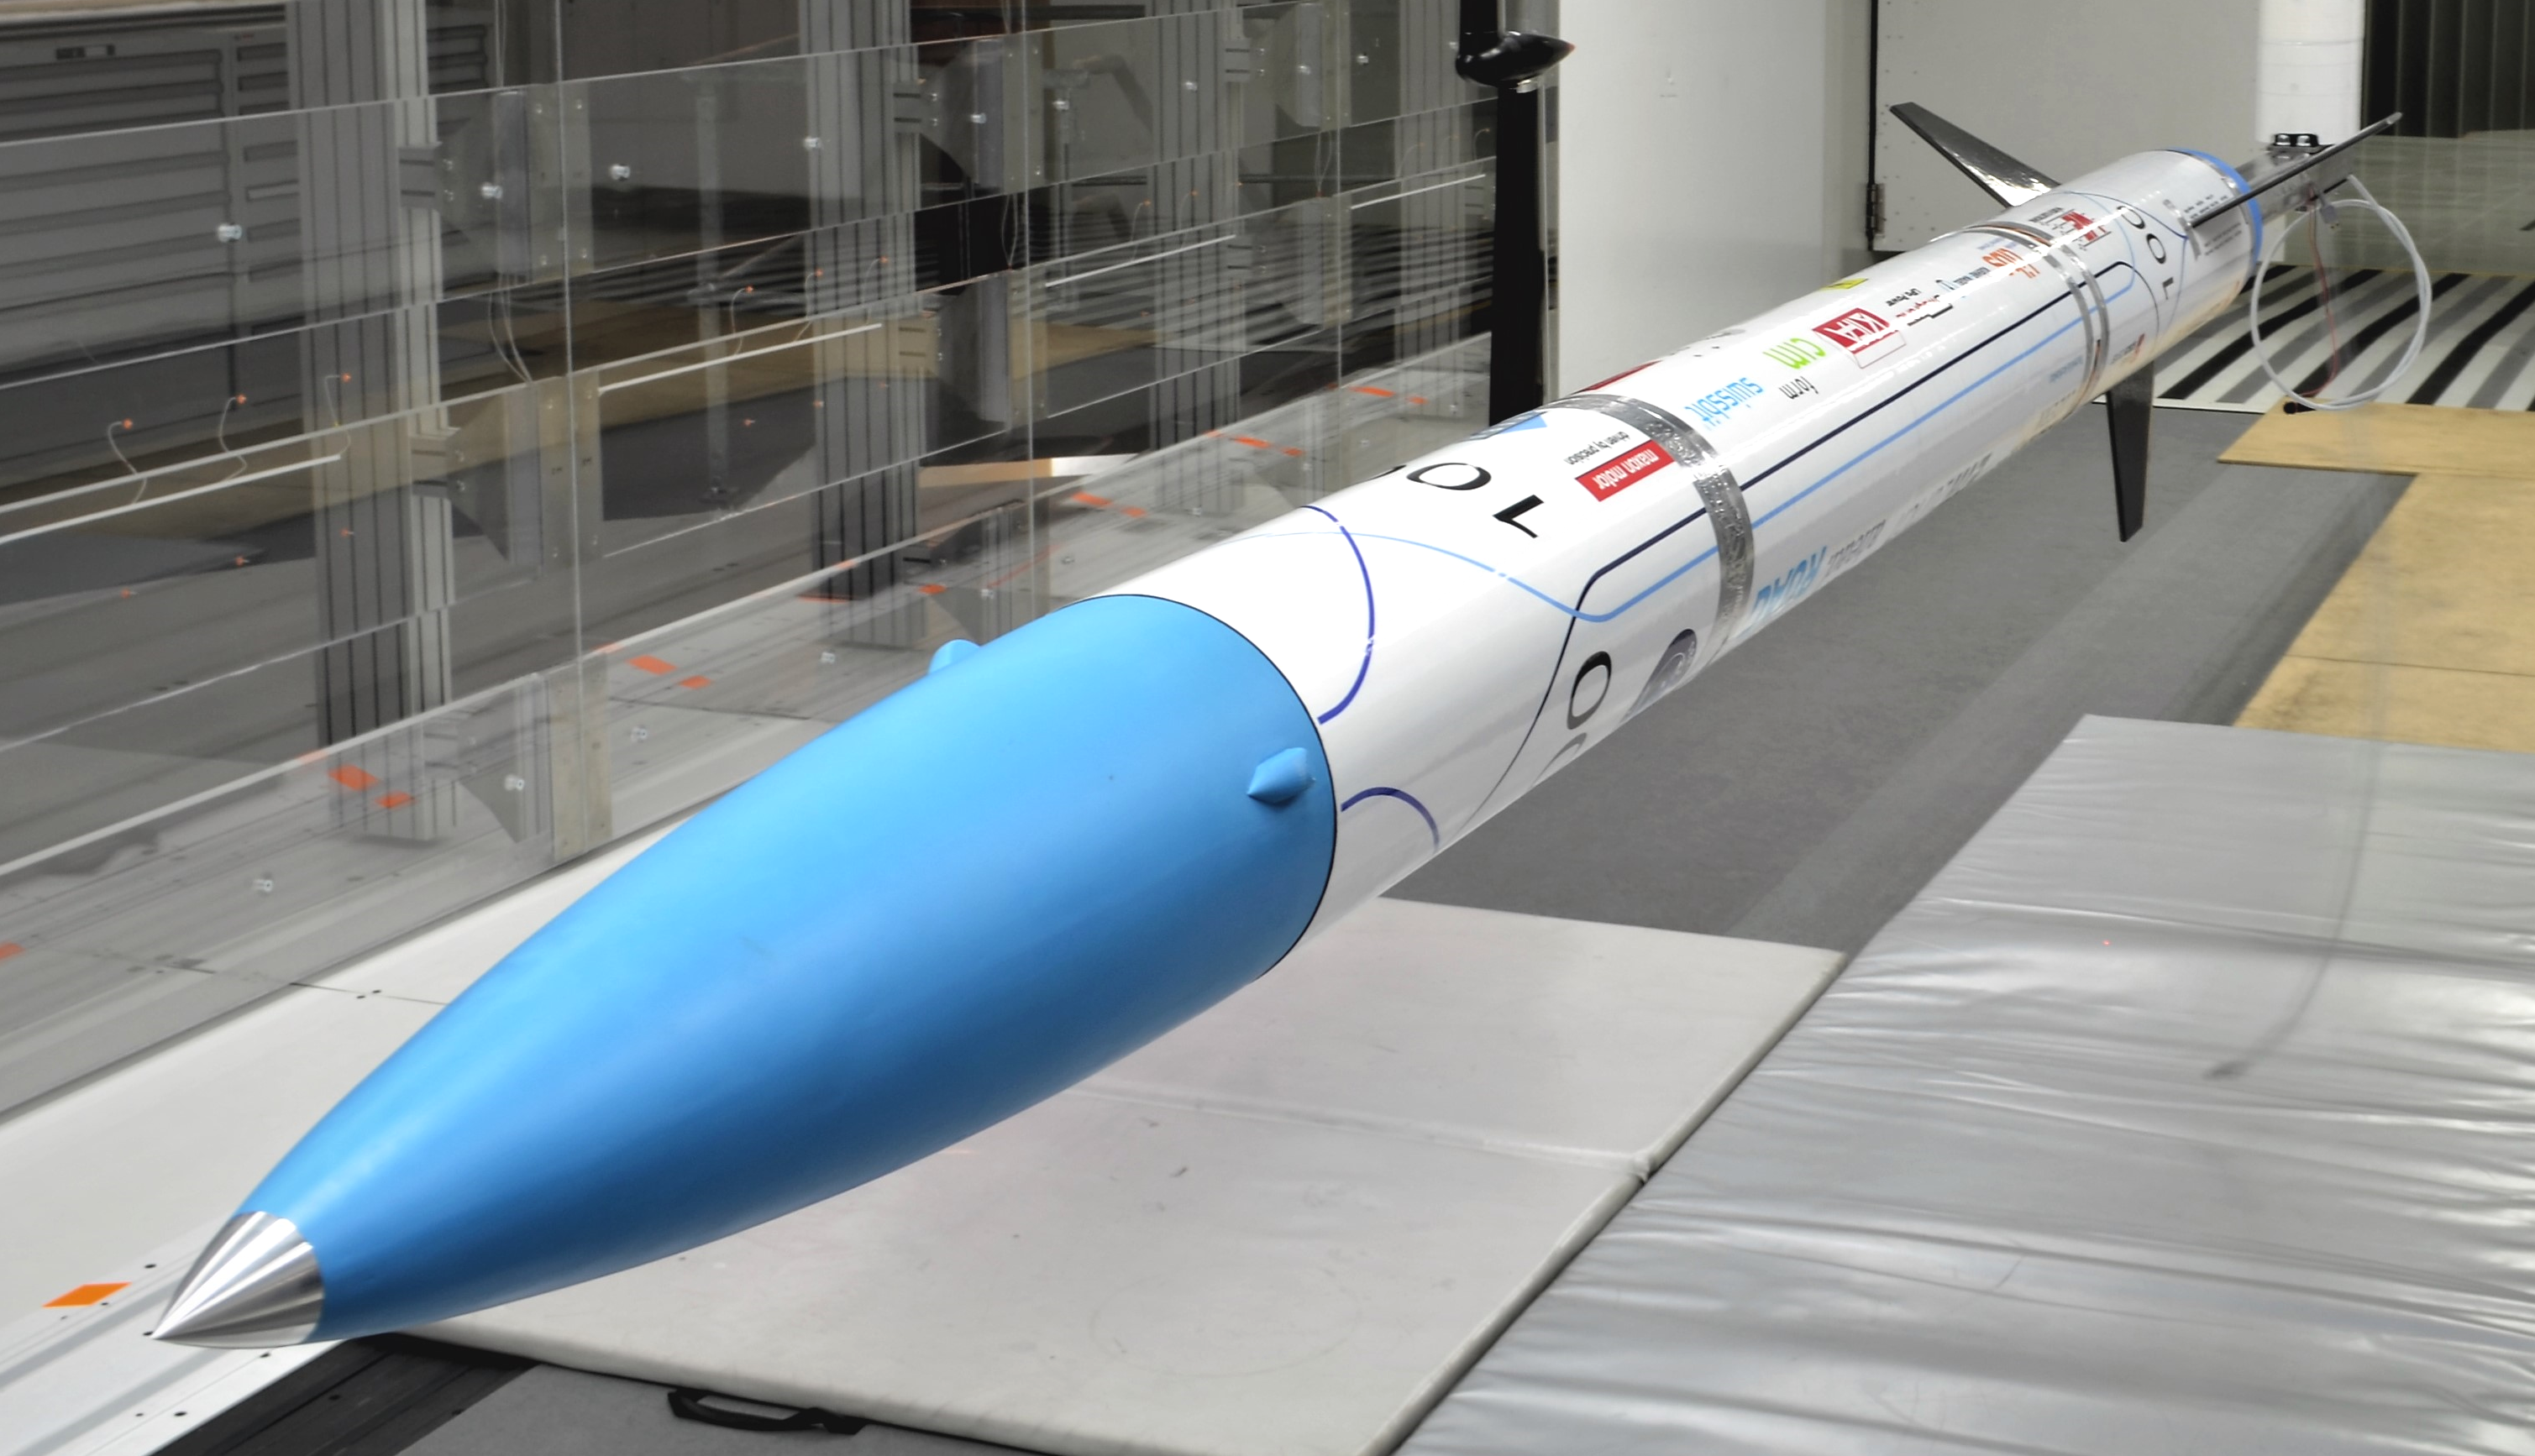
\includegraphics[height=6cm]{images/TELL_1.png}
 \caption{TELL \rom{1} in the wind tunnel}
 \label{fig:tell_1}
\end{figure}

The avionics on the rocket are split into the two parts nose cone avionics and lower body avionics as shown in figure \ref{fig:tell_structure}.
Both parts are the same apart from the GPS and telemetry in the nose cone, and two additional barometers, rocket motor temperature sensor and payload interface for the lower body avionics.
Sensors that both parts have separately are an accelerometer, magnetometer, gyroscope and climate sensor.
Both parts also log their collected data to a separate SD card.
This is done to have redundancy and to be able to have sensors in all parts of the rocket.
The two parts are connected over a wireless link to be able to communicate after the nose cone is popped off at the first recovery event.
The central component of each avionics module is an ARM M4 microcontroller that acts as the flight controller.
It connects to all the sensors and communication modules of its half of the rocket.

The nose cone avionics has two GPS antennas with a separate receiver for each.
One is directed upwards to have reception in the time from launch to the apogee.
The other is directed downwards to have reception after the nose cone is hanging upside down after the first recovery event.
The telemetry transmitter and antenna are also implemented in the nose cone.
For the transmitter, the XBee-PRO SX module is used.
It transmits on the frequency band from 902 to 928 MHz, which is open for public use in north america, where the competition is taking place.
With a transmitting power of 1 W, it can establish a link over a range of up to 105 km.

\begin{figure}[ht]
 \centering
 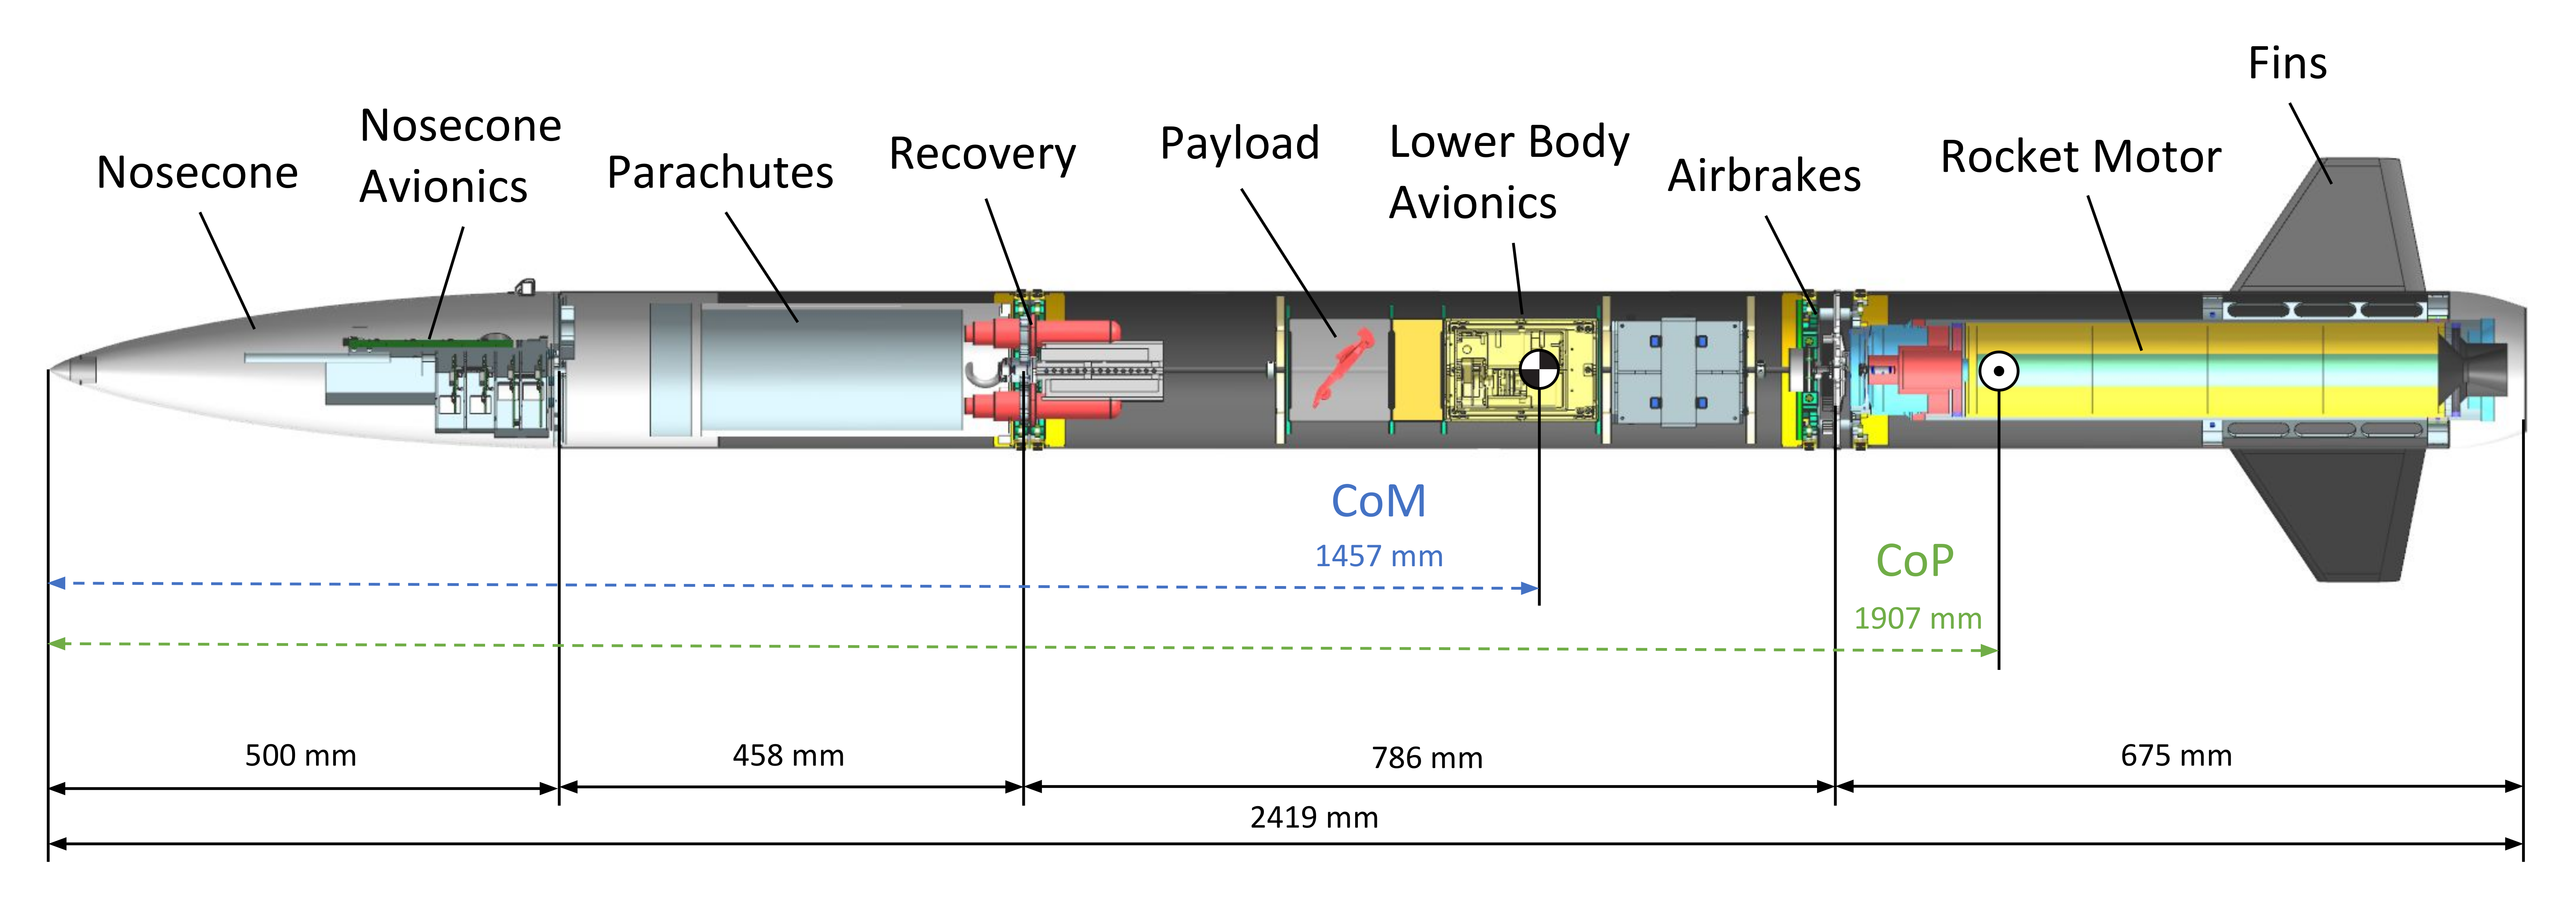
\includegraphics[width=\textwidth]{images/TELL_Structure.png}
 \caption{Overview of TELL}
 \label{fig:tell_structure}
\end{figure}

\subsection{The Ground Station}

The central part of the ground station is the a laptop that displays the live flight metrics.
Connected to it over USB is a second XBee module, that receives the telemetry data sent by the rocket.
A directional antenna is used to receive the downstream.

In this years project, it is planned to do post-processing DGPS to analyze the trajectory.
GPS raw data has to be logged on the rocket and at a reference station in order to do that.
For post-processing DGPS, no data link is needed to the rocket.
A GPS receiver is placed at the ground station to act as the reference station.
The GPS module M8T from u-blox was chosen for this purpose and is used in the rockets nose cone avionics, as well as at the ground station.
The speciality of the M8T module is, that it provides raw GPS data like the measured pseudoranges.
This is needed for post-processing DGPS.


\section{System Overview}\label{sec:system_overview}

The difference of the DGPS system described in this thesis to the post-processing one used by project TELL is when the corrected position is available.
A real-time system is needed that the corrected position can be directly used to control the rocket.
This adds the requirement for a live PRC calculation, a data link to the rocket, and the inclusion of the corrections into the position estimation on the rocket.

Let's start with the data link.
Is is needed to send the corrections from the reference station, which is in this case the ground station, to the rocket.
With the telemetry system, a link is already established.
Although this is only a downlink for project TELL, the used XBee modules can be configured for a two way communication link.

For the DGPS to work, the measured pseudoranges on the rocket have to be corrected with the PRCs before they are used to estimate the position.
There are two possible ways to achieve this.
For the first way, the receiver would have to provide raw GPS data to the flight computer where the PRCs can be added.
The position would then have to be estimated outside the receiver by the flight computer.
The challenge with this approach is, that the implementation of a position estimation algorithm from raw GPS data is huge development effort, especially on a microcontroller.
The second way is to choose a GPS receiver that accepts PRCs in a certain format and includes them in its position estimation.
This method has the advantage of a much smaller development effort because the position estimation can be left to the receiver.
The drawback is that the specific DGPS protocol accepted by the receiver has to be used, which limits the design freedom.
Both methods are possible with the current M8T GPS receiver.
It was specifically chosen because it outputs raw GPS data like the pseudoranges.
It also accepts PRCs in the form of an RTCM data stream, which is described in section \ref{sec:rtcm}.
The second approach, where the receiver estimates the position, was chosen for this project to make it feasible to implement.
There are other receivers besides the M8T that have this functionality.
The selection of the receiver is addressed in section \ref{sec:receiver}.

Finally, the PRCs have to be generated at the ground station.
A similar trade-off between flexibility and small development effort as for the position estimation in the rocket has to be made here.
The PRCs can either be calculated from GPS raw data, or a receiver with integrated reference station functionality can be used.
The decision was made in favor of a custom reference station algorithm.
The development effort is not as big as for a position estimation algorithm.
Also, such a system can more easily be implemented in parallel to the current post-processing DGPS method, which will always be more precise than a real-time solution for post-flight analysis.
The custom application developed to generate the PRCs is described in section \ref{sec:dgps_message_generator}.

\begin{figure}[ht]
 \centering
 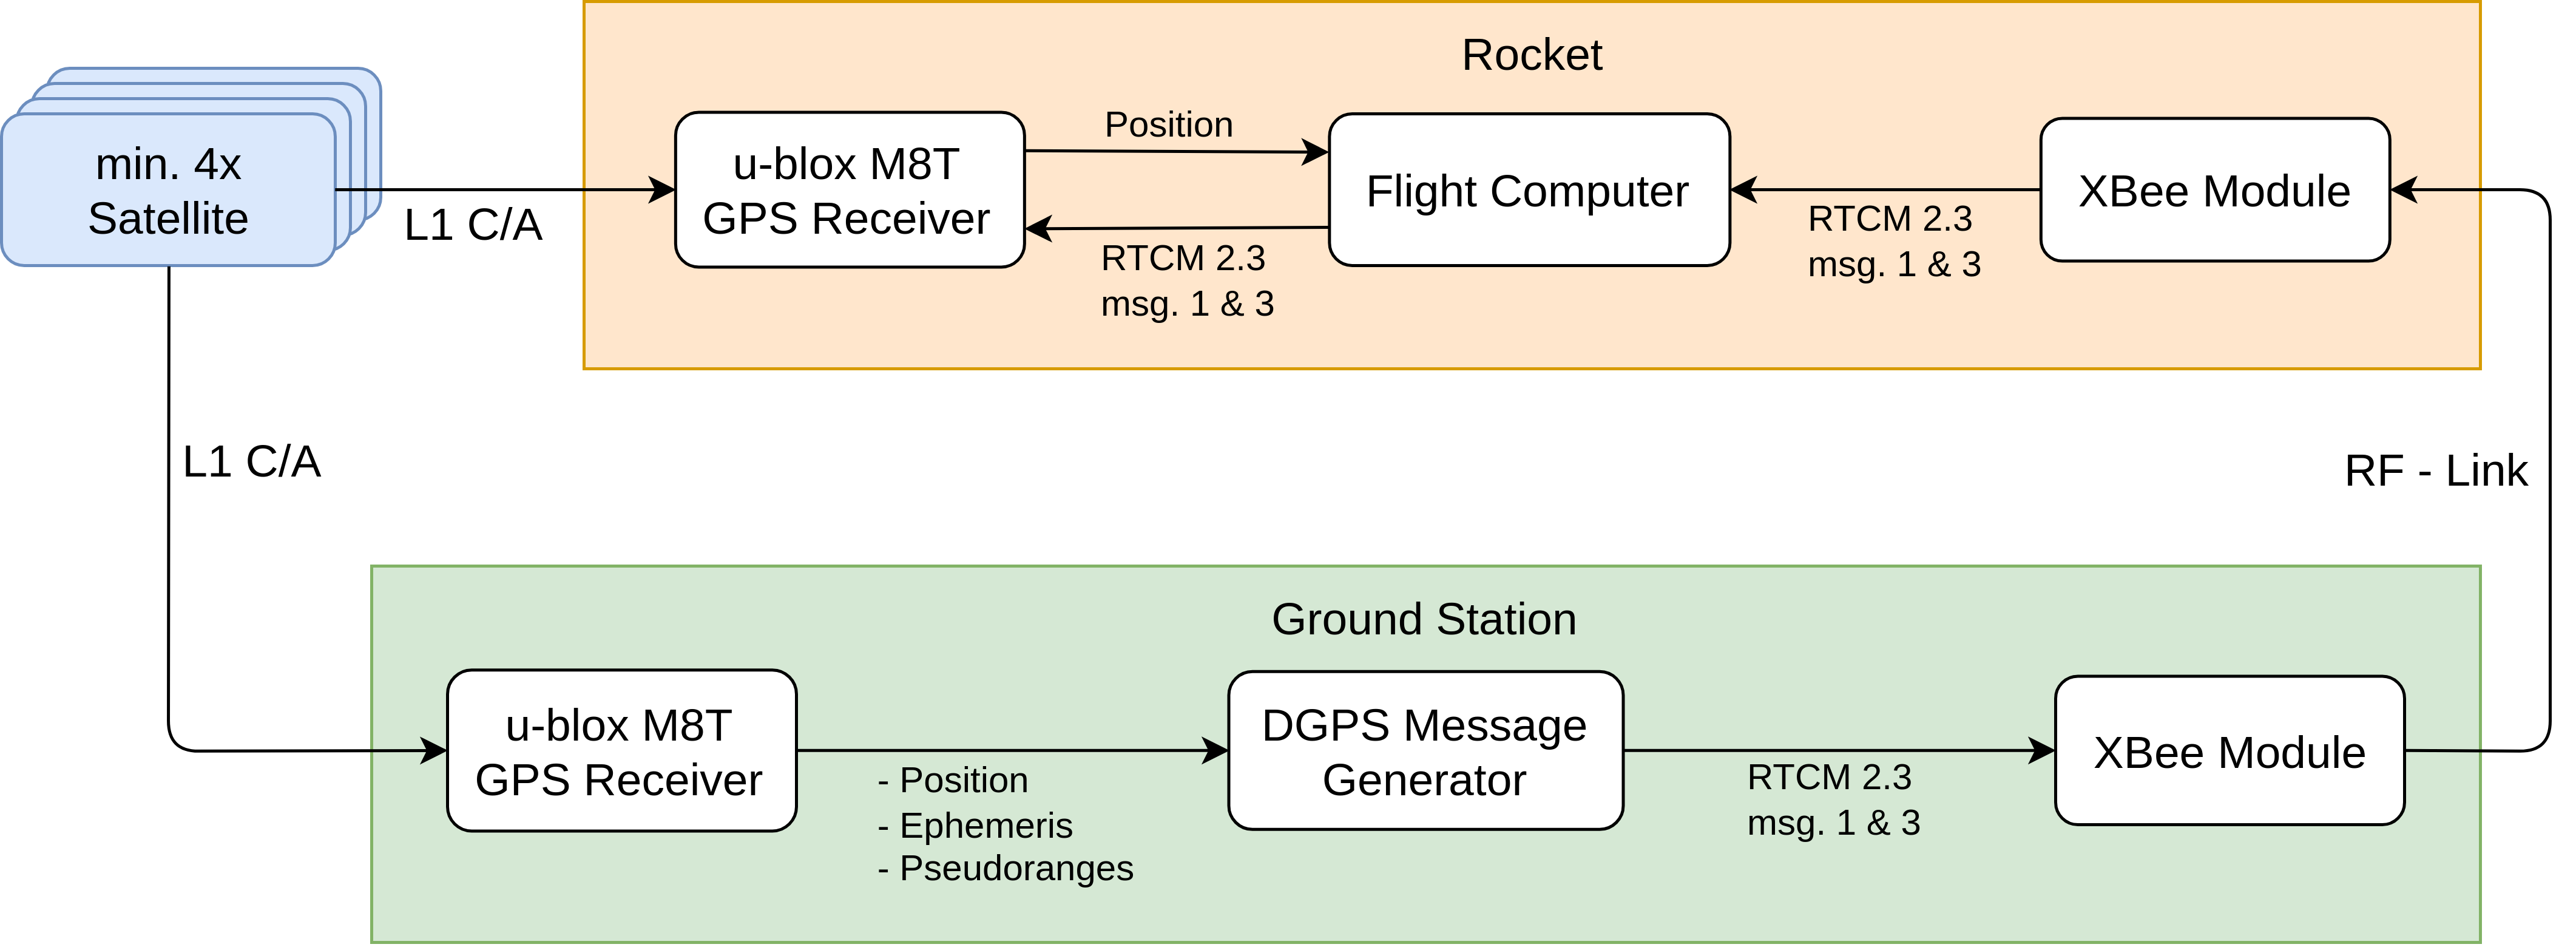
\includegraphics[width=\textwidth]{images/DGPS_System_Overview.png}
 \caption{DPGS system overview}
 \label{fig:dgps_system_overview}
\end{figure}

A top level view of the data flow for the planned system is shown in figure \ref{fig:dgps_system_overview}.
It starts with the generation of the GPS signals by the satellites.
The standard L1 C/A signals are used.
Both receivers have to receive the signals from a set of at least four satellites for the system to work.
The receiver at the ground station then measures the pseudoranges, decodes the navigation messages, and estimates its position.
It then sends its position, the navigation message bits which include the ephemeris data, and the measured pseudoranges to the ground station laptop over a USB connection.
This data is processed by the custom DGPS message generator application running on the ground station laptop.
The calculated PRCs are packed in messages of the RTCM 2.3 standard.
Message 1 and 3 of the standard are needed by the M8T receiver.
They are sent over another USB connection to the XBee module of the ground station to be transmitted over the RF link to the rocket.
The messages are forwarded to the flight computer in the nose cone, where they are separated from other data and fed into the GPS receiver on the rocket.
This receiver then corrects its pseudoranges with the latest PRCs before estimating the rocket position.


\section{GPS Receiver}\label{sec:receiver}

\begin{minipage}{0.6\textwidth}
  A seen in figure \ref{fig:dgps_system_overview}, the M8T receiver from u-blox used by TELL was also chosen for this project.
  The reasons for this decision were the following:
  \begin{itemize}
  \item output of raw GPS data
  \item support of the RTCM 2.3 standard
  \item same receiver can be used for rocket and reference station
  \item compatibility with post-processing DGPS
  \end{itemize}
  The avionics of project TELL are modular with separate boards for telemetry, GPS, and intra-rocket communication.
  This reduces the development effort and faulty parts can be replaced more easily.
  The different boards are connected with RS232 interfaces.
  Figure \ref{fig:m8t_receiver_board} shows the GPS board with a M8T receiver, antenna connector, RS232 interface, USB interface, and 12 V input.
  This board is used twice in the rocket and once at the ground station as post-processing DGPS reference station for project TELL.
  The exact same hardware setup can be used for the real-time DGPS.
\end{minipage}
\hfill
\begin{minipage}{0.37\textwidth}
 \centering
 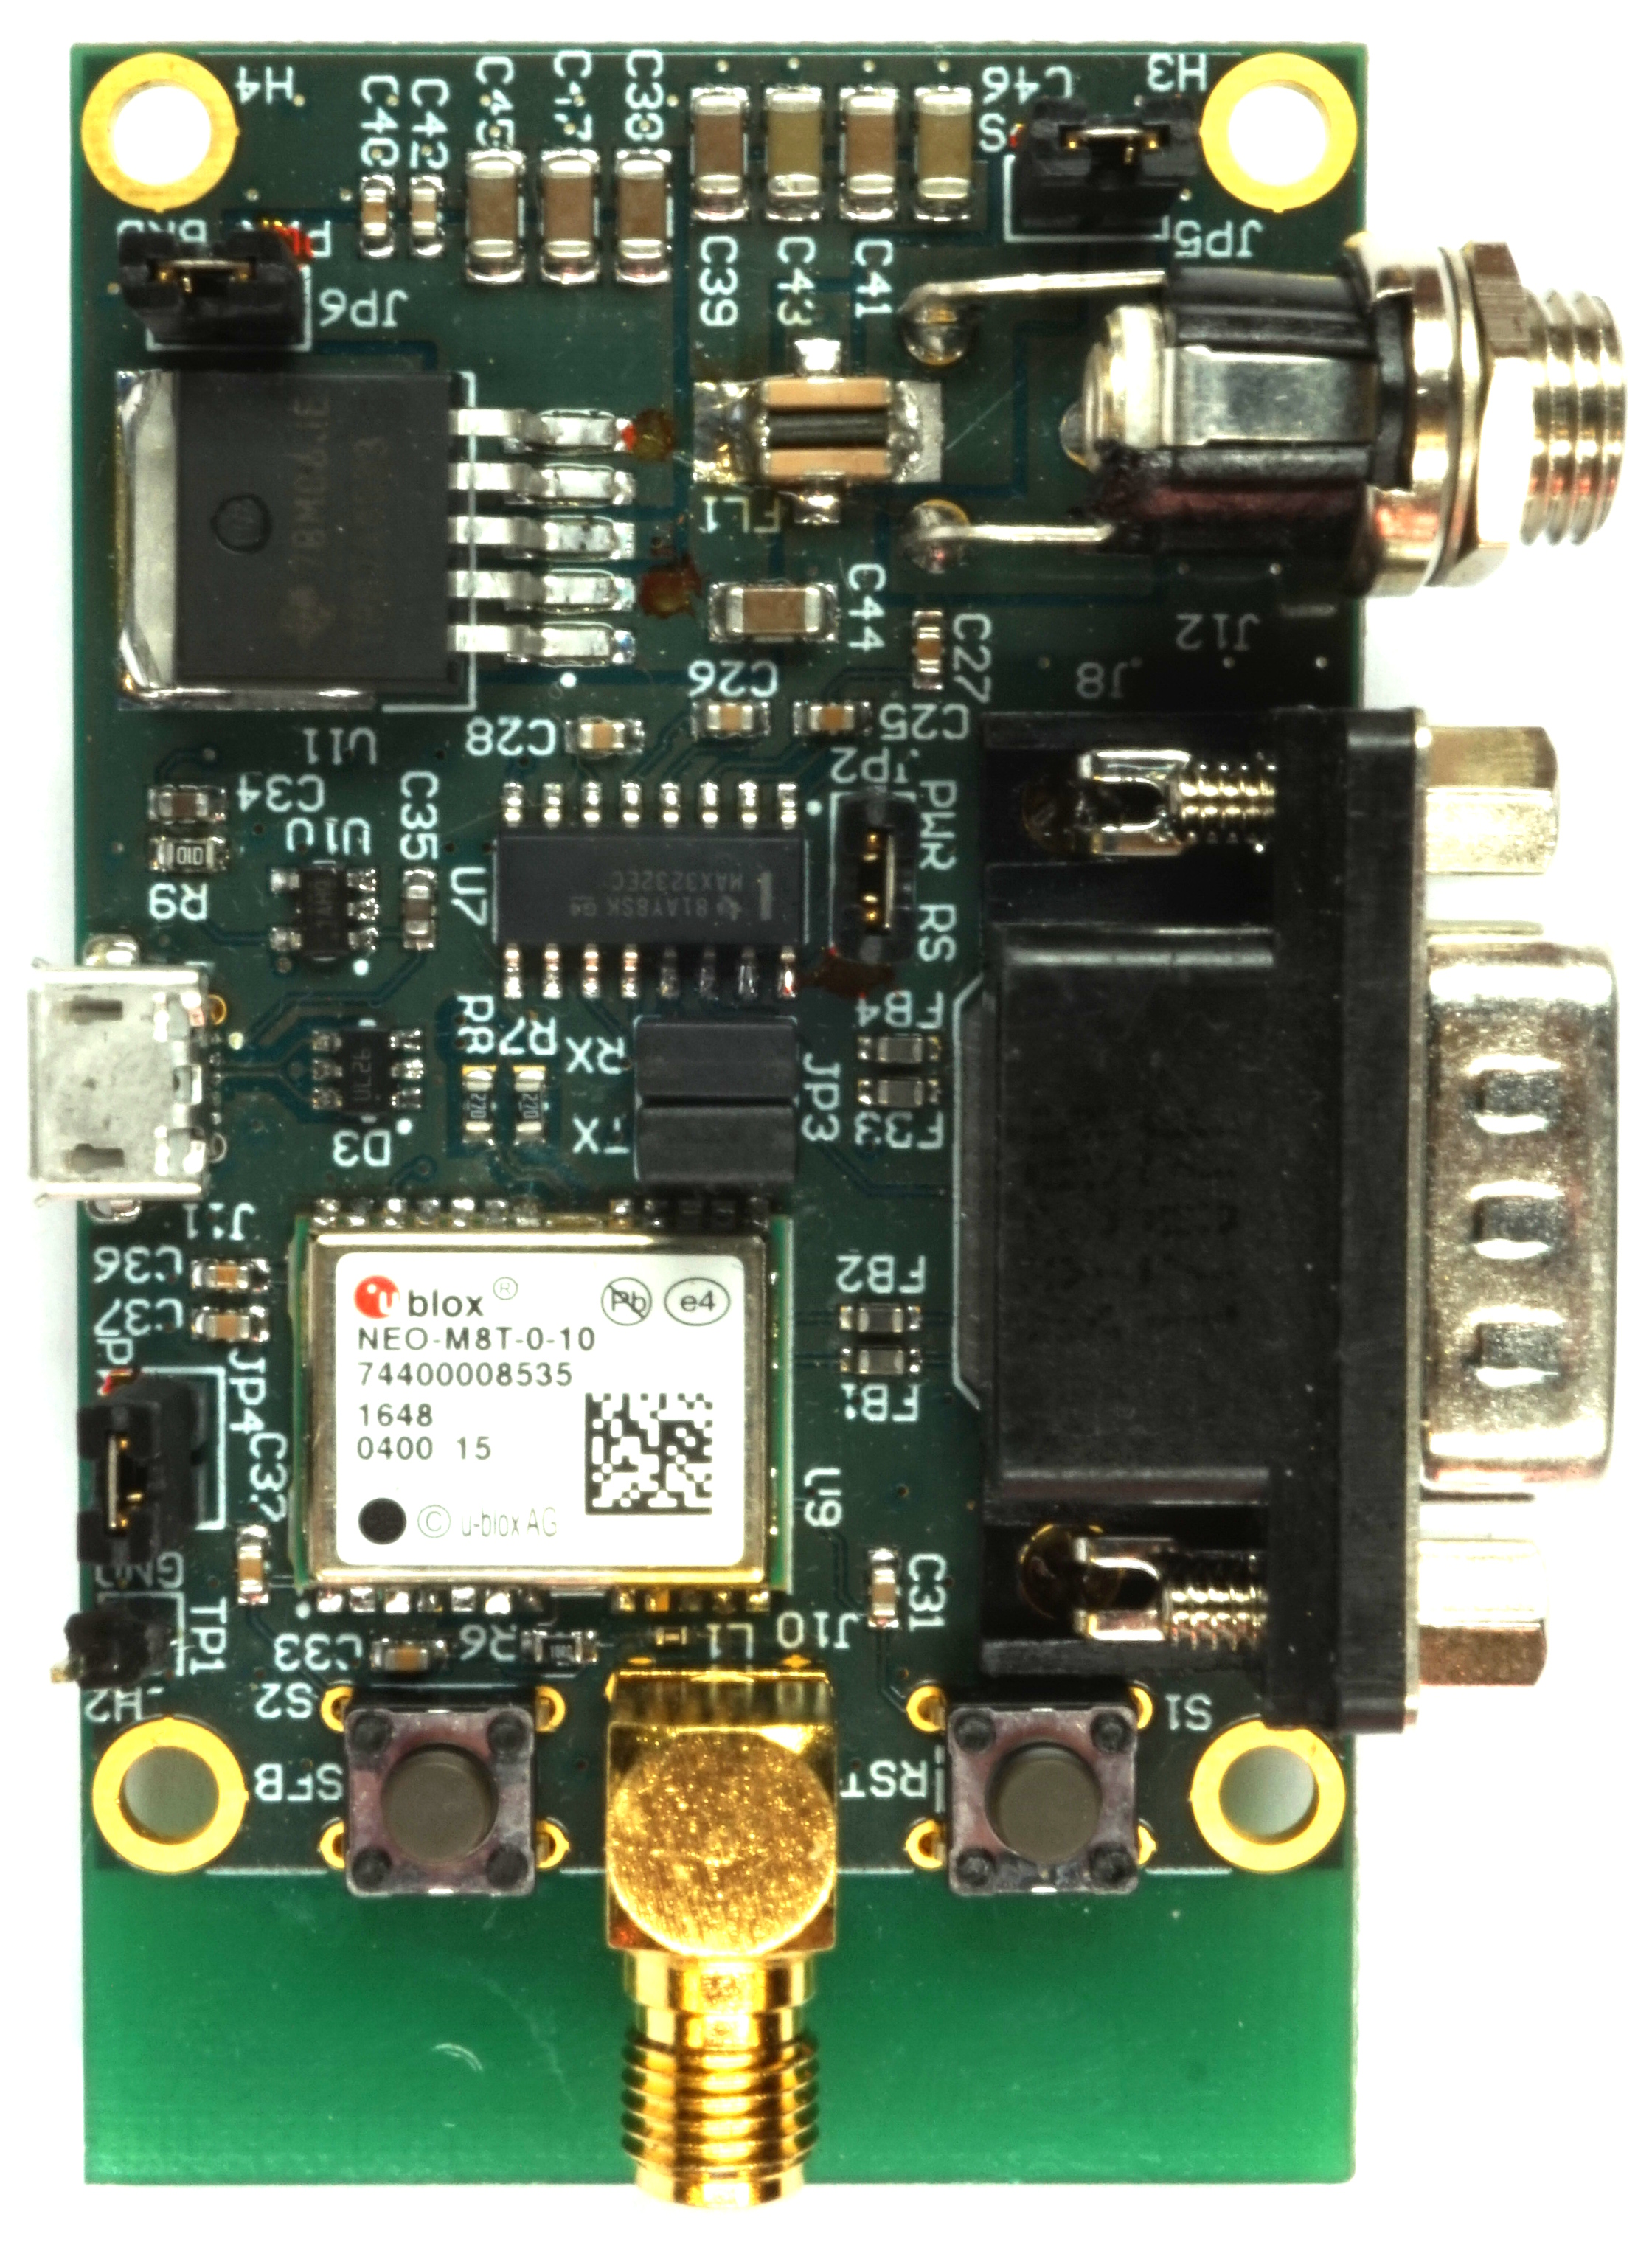
\includegraphics[width=\textwidth]{images/M8T_Receiver_Board.jpg}
 \captionof{figure}{GPS board of project TELL with u-blox M8T receiver}
 \label{fig:m8t_receiver_board}
\end{minipage}

GPS receivers from u-blox can communicate with messages from three different protocols.
The first one being NMEA.
It is the standard way for GPS receivers to output their data.
It is in ASCII format which makes it easy to extract the messages from a data stream.
All the standard data like time, position and satellite information can be acquired with NMEA messages.
The second is the u-blox proprietary UBX protocol.
Much more specific information can be obtained with UBX messages like the GPS raw data in the case of the M8T receiver.
It is also used to configure the receiver.
The third protocol understood by u-blox receivers is RTCM.
It is a set of standards for receiver independent differential GPS corrections.
It is described in section \ref{sec:rtcm}.

A requirement for the receiver on the rocket is that the acceleration, velocity and altitude experienced on a sounding rocket do not exceed its operational limits.
The operational limits of 50'000 meters max. altitude and 500 m/s max velocity of the M8T receiver are both sufficient.
The goal of the competition is to go to an altitude of 3048 meters.
The max. speed reached by TELL will be at the border to supersonic which is 343 m/s.
Those are legal limits where the receiver must not provide a fix if exceeded.
The acceleration limit on the other hand is caused by the implementation of the receiver.
It is only 4 g, whereas TELL will experience up to 10 g of acceleration.
This could pose a problem.
But the receiver is actually not required to get a fix during the burn when the acceleration is experienced.
It only has to get a fix max. 2 seconds after burnout.
If the reaquisition time is sufficiently small, the receiver could still meet the requirements.
This parameter is not given in the datasheet, but the related parameter of a time-to-first-fix in case of a hot start is given as 1 second.
If this requirement will be met can only be definitively confirmed with a rocket flight test. \cite{M8T}


\section{RTCM 2.3 Standard}\label{sec:rtcm}

RTCM stands for Radio Technical Commission for Maritime Services.
It is an organization that defines standards mainly for use in maritime applications.
One group of standards defines the protocol for DGPS corrections.
There are three generations of standards in this group.
The most recent ones being 10403.3 of the third generation and 10402.3 of the second generation.
U-blox GPS receivers with the possibility of DGPS understand either of those standards.
In the case of the M8T it is 10402.3 which is mostly just called RTCM 2.3 \cite{RTCM_2.3}.

The RTCM 2.3 standard defines 30 messages.
The messages are divided into 30 bit long words like the GPS navigation messages.
The last 6 bits of each word are parity bits.
The parity algorithm is also adopted from the GPS navigation messages and can be found in the GPS Interface Specification \cite{IS-GPS-200}.
It defines that the parity of each word is connected to the last two parity bits of the previous word.
This is also true across messages for the RTCM 2.3 standard.
Each message starts with a header of two words that includes a preamble, the message type, the station I.D., a modified version of the z-count (time reference in navigation messages), a sequence number, the number of data words in this message, and the station health.

The M8T receiver requires message 1 and message 3 to enter DGPS mode.
Message 1 is used to transmit the DGPS corrections.
For each satellite a PRC is calculated, this message transmits a scale factor, user differential range error (UDRE), pseudorange correction, range-rate correction, and issue of data (IOD).
The scale factor determines the scale of the pseudorange correction to 0.02 or 0.32 m and the range-rate correction to 0.002 or 0.032 m/s.
The UDRE is the estimated error in the differential corrections.
The range-rate corrections can be used to interpolate between pseudorange corrections.
It is no longer necessary since Selective Availability (an intended noise introduced to civil GPS signals) was switched off in the year 2000, and can be set to 0.
The IOD is sent to ensure that both the reference station and the user use the same parameters to calculate the satellite position.
Message three transmits the XYZ coordinates of the reference station in the WGS84 reference frame.
This message is needed to determined the closest reference station if multiple RTCM streams are received.

It is important for the system to work that both the reference station and the user correct the pseudoranges for the same errors.
The standard states that the raw pseudoranges have to be adjusted for the receiver clock offset, satellite clock offset, satellite relativistic corrections, and L1-L2 group delay correction in the case of a dual frequency receiver.
Neither of the atmospheric errors should be modeled to correct the pseudoranges.
Only a tropospheric model that incorporates the different altitudes of the reference station and user can be applied if necessary.
For the data link, an update rate of once every 30-60 seconds is stated as adequate.


\section{DGPS Message Generator}\label{sec:dgps_message_generator}

It was decided to develop a custom application to generate the PRCs from the raw GPS data at the reference station.
This made up the biggest part of the development effort for this project.
The application has to run on the ground station laptop and connect to the GPS receiver as input and the XBee module as output.
It was written in C++ and developed to run on Linux.
For the development environment, Qt Creator was chosen.

\newpage

\subsection{Software Architecture}

The different files of the application and their connections are shown in figure \ref{fig:software_architecture}.
On application startup, the MainWindow widget starts running.
It is responsible for the graphical user interface (GUI) and the start of the underlying programs.
Before the DGPSMesGen can be started, the application has to know the location of the reference station.
This position can either measured with the PositionAveraging, or it can be loaded from a file or from the RefPosDialog.
When the reference position is set, the DGPSMesGen can be started.
It then starts the UBloxInterface, XBeeInterface and NavMessageDecoder.
The DGPSMesGen and the three newly started threads communicate over multiple instances from the ThreadQueue class.
The data types used to transmit data over the ThreadQueues are defined in the header files GPSDataTypes and UBloxMessages.
Additional functions used by the UBloxInterface and XBeeInterface are implemented in the files TypeConversion and RTCMEncode.
A Debug header file is used to enable debug and logging functionality.

\begin{figure}[ht]
 \centering
 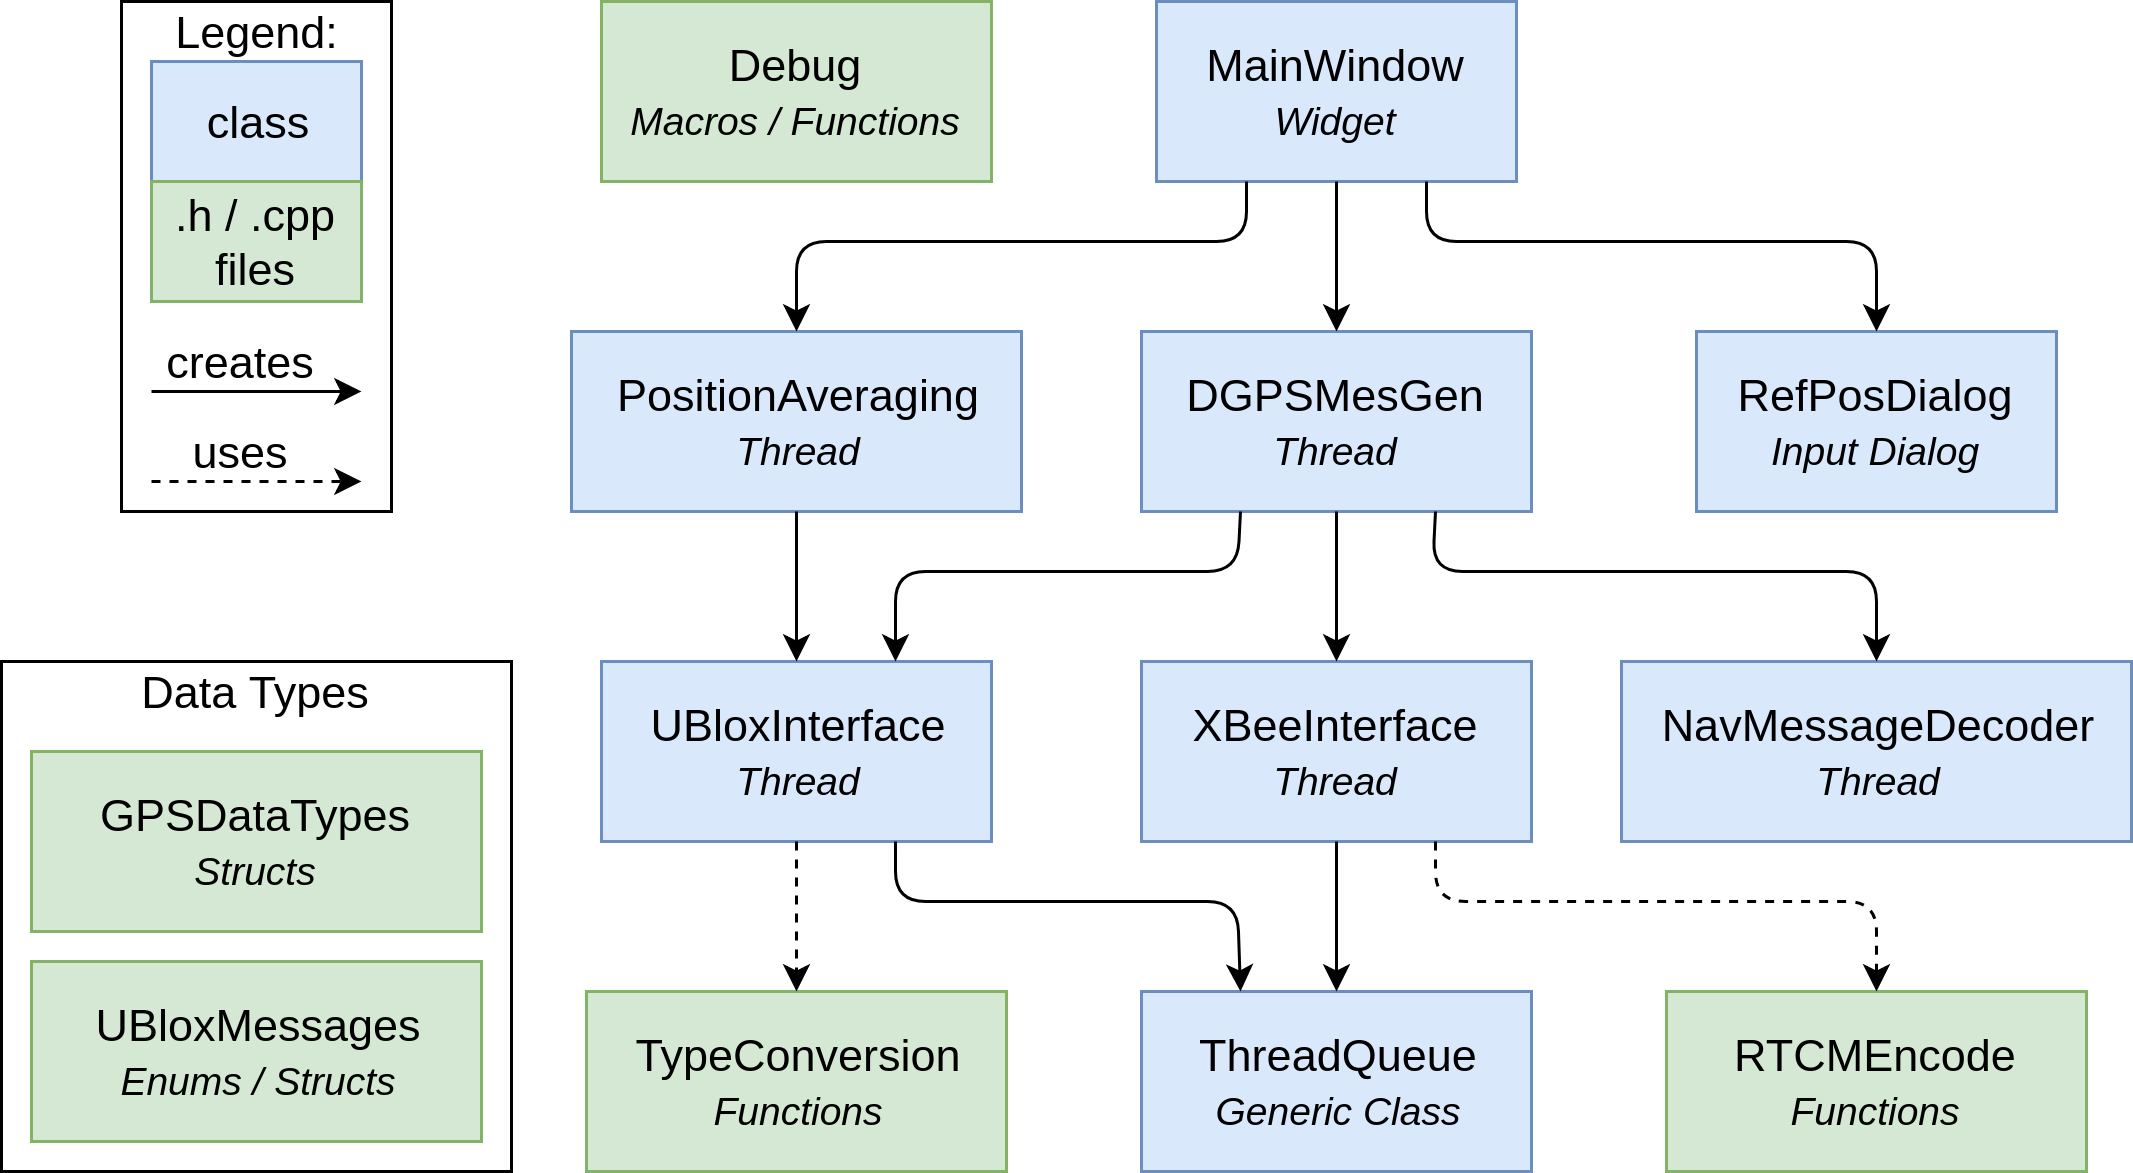
\includegraphics[width=\textwidth]{images/Software_Architecture.png}
 \caption{Software architecture of the DGPS Message Generator}
 \label{fig:software_architecture}
\end{figure}

\subsection{Data Flow}

The data flow graph in figure \ref{fig:data_flow} gives a better overview of the internal functionality of the DGPS Message Generator and how it fits into the ground station infrastructure.
The data stream from the GPS receiver is channeled over a USB port of the laptop to a serial port, from where it can be read from the application.
The UBloxInterface reads the serial stream and extracts the needed messages.
Two ThreadQueues are fed with the messages containing the pseudoranges and the navigation messages.
The Navigation Message Decoder pulls the raw navigation messages from the ThreadQueue and extracts the ephemeris and other satellite data.
If a pseudorange measurement and all needed satellite data is available, it is processed by the DGPS Message Generator and incorporated in the next correction message.
All the data needed to generate the RTCM message 1 and 3 are forwarded to the XBee Interface.
That is where the data is encoded into the RTCM protocol and then sent out to an XBee application also running on the laptop.
It routes the data over a serial port and USB port to the XBee module.

\begin{figure}[ht]
 \centering
 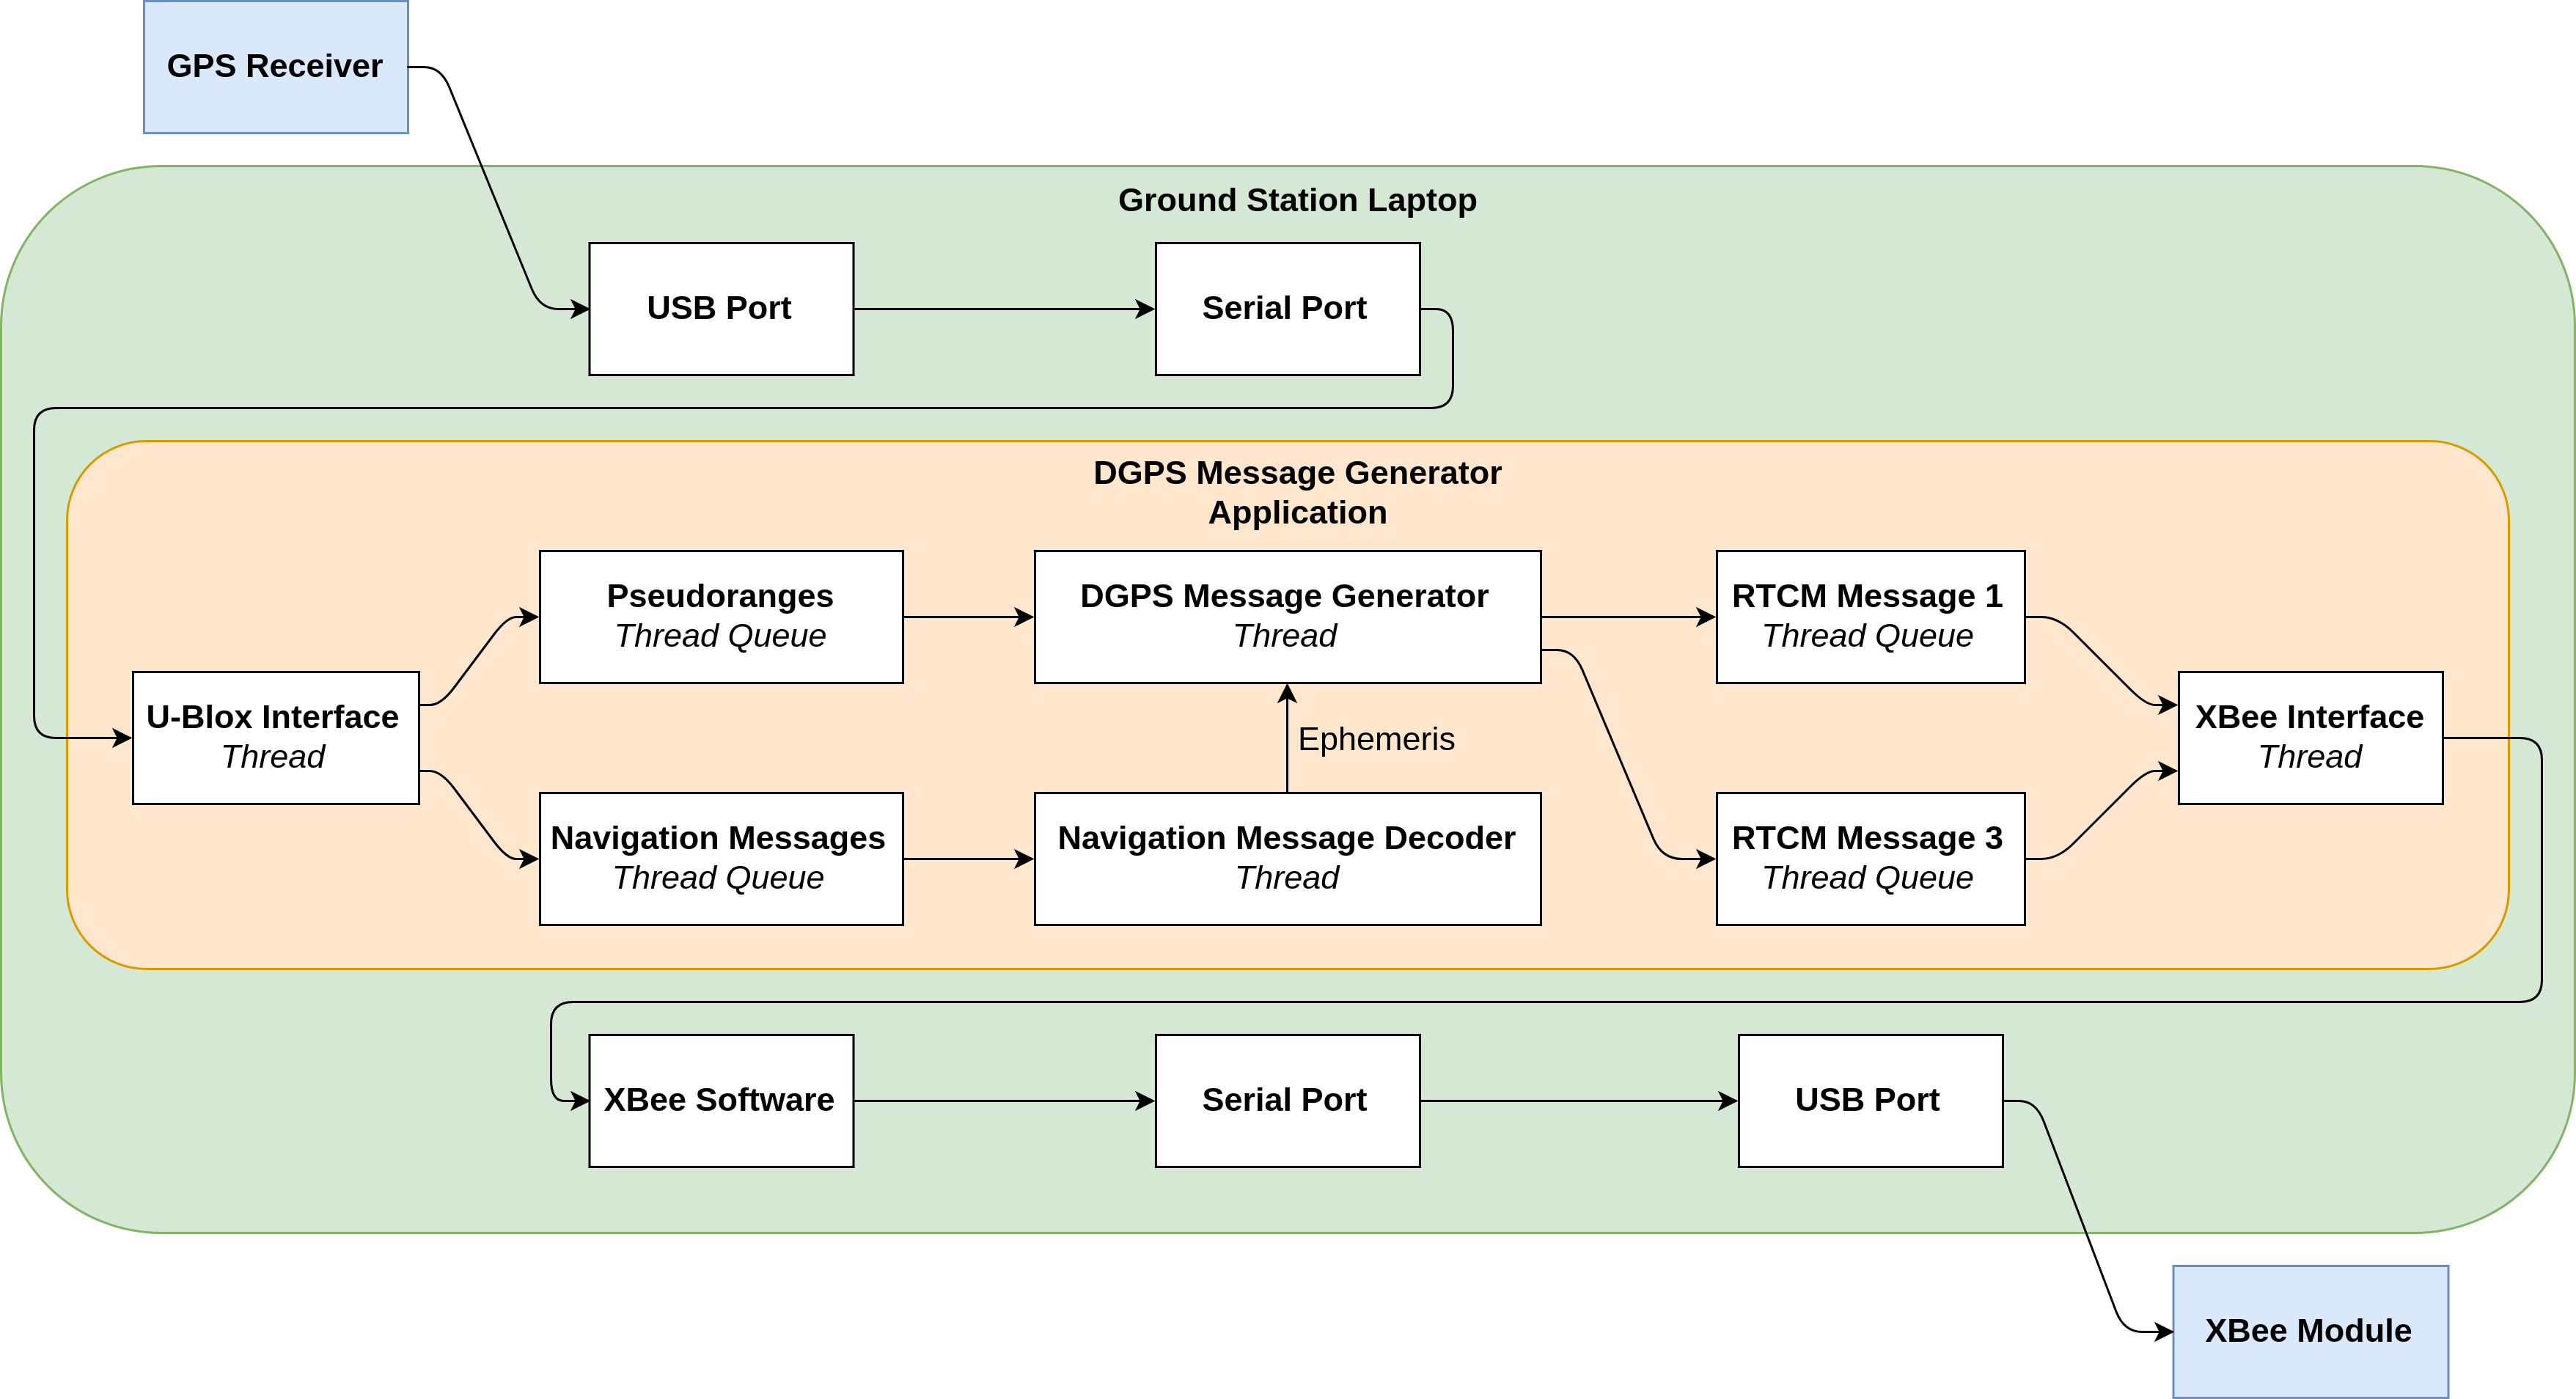
\includegraphics[width=\textwidth]{images/Data_Flow.png}
 \caption{Data flow from the GPS receiver to the XBee module}
 \label{fig:data_flow}
\end{figure}

\subsection{Graphical User Interface}

\begin{minipage}{0.5\textwidth}
 The front end of the application is a graphical interface.
 On the top, it has multiple options to set a reference position.
 It can be set directly over an input dialog (Set), loaded from a file (Load) or measured with a connected GPS receiver (Measure).
 The current reference position can also be saved to a binary file with the ending .wgs84 for later use (Save).
 The middle section is a sort of command line output.
 All actions made by the user are confirmed there and errors are displayed in red.
 On the bottom, the actual DGPS Message Generator can be started and stopped.
 Input and output port and baud can be specified here.
 The output settings are only needed if the external XBee software is bypassed and the RTCM messages are directly sent to a serial port.
\end{minipage}
\hfill
\begin{minipage}{0.45\textwidth}
 \centering
 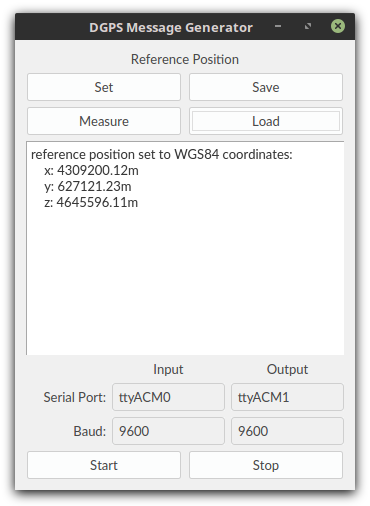
\includegraphics[width=\textwidth]{images/GUI.png}
 \captionof{figure}{Graphical user interface}
 \label{fig:gui}
\end{minipage}

\subsection{U-Blox Interface}

The communication with the GPS receiver takes place over the proprietary UBX messages.
Three messages are needed by the application.
The pseudoranges are transmitted with the UBX-RXM-RAWX message.
The GPS navigation messages are transmitted in raw form by the UBX-RXM-SFRBX message.
To be able to measure the reference position, the UBX-NAV-POSECEF message is used.
It has the information of the position estimation in ECEF form.

The bytes for each value of a message are read from the serial port and converted to the their original data type using functions from the TypeConversion header file.
All the values of a message are then combined in a struct and pushed to the appropriate ThreadQueue.

When the thread starts, UBX configuration messages are sent to the GPS receiver to set the operation mode and enable the needed messages.
The UBX-RXM-RAWX and UBX-NAV-POSECEF messages then come in with a frequency of 1 Hz.
UBX-RXM-SFRBX is sent when navigation message data is available in the GPS receiver.

The reception and conversion to the right data types of all three UBX messages works as expected.
The integrity of the values has been checked with the u-blox evaluation software u-center.

\subsection{Position Averaging}

One option to set the reference position is by measuring it directly with the GPS receiver.
This position will be biased by the GPS errors.
To get a more accurate position, the position is measured over a period of time and then averaged.
When the Measure button on the GUI is pressed, the PositionAveraging thread is started.
It saves all the position values form UBX-NAV-POSECEF messages that come in over the UBloxInterface in a vector until the Measure button is pressed again.
All the values in the vector are then averaged and set as new reference position.

\subsection{Navigation Message Decoder}

The NavMessageDecoder thread is started in parallel to the DGPSMesGen thread.
It is responsible for the decoding of the GPS navigation messages.
Their content is needed by the DGPSMesGen to calculate the satellite positions and the satellite clock corrections.
It starts by reading the UBX-RXM-SFRBX messages.
They contain the raw navigation messages.
The values are extracted from the byte values much like the UBX messages in the UBloxInterface.
Navigation messages come in subframes.
The first three subframes of the navigation message of a satellite are needed to calculate its position and clock correction.
When a subframe is decoded, the values are saved to the appropriate ephemeris struct.
When an ephemeris struct has the matching information of all three subframes, it is marked as valid.
A valid ephemeris struct can be fetched by other threads with the public getEphemeris function.

The navigation messages are usually updated every two hours.
If the parameters are being extracted correctly has been checked with a comparison to the ephemeris and clock values provided by IGS \cite{IGS}.

\subsection{DGPS Message Generator}

In the DGPSMesGen thread, the actual PRCs are calculated.
It waits until a UBC-RXM-RAWX message is available from the ThreadQueue.
If ephemeris data is available from the NavMessageDecoder for the pseudoranges in the RAWX message, it continues to calculate the PRCs for those satellites.
It iterates trough all satellites for which a pseudorange and ephemeris data is available.
The calculation for each satellite is done in the following steps:
\begin{enumerate}
 \setlength\itemsep{0.1cm}
 \item calculate the time of transmission: \\
 time of transmission = time of reception - transmission time
 \item calculate the satellite position at the time of transmission and correct it for the earth's rotation during transmission
 \item calculate the distance between reference station and satellite: \\
 calculated range = $\lvert \lvert$ reference position - satellite position $\rvert \rvert$
 \item calculate the satellite clock correction: \\
 satellite clock correction = satellite clock offset + satellite relativistic correction
 \item correct the raw pseudorange with the satellite and receiver clock corrections: \\
 corrected pseudorange = raw pseudorange + (satellite clock correction + receiver clock offset) $\cdot$ speed of light
 \item calculate the pseudorange correction: \\
 pseudorange correction = calculated range - corrected pseudorange
\end{enumerate}
After all pseudorange corrections are calculated, the receiver clock offset is estimated.
This is done by taking the average of the pseudorange corrections: \\
receiver clock offset = mean(pseudorange corrections)

Because the receiver clock offset is not available yet when the pseudorange is corrected, the whole process has to be done iteratively.
It is implemented with three iterations to get a good receiver clock offset estimation.
After this, the PRCs are smoothed with a moving average filter.
The filter is configured to average over ten values.
The filtered PRCs along with their satellite ID and IOD are pushed to the ThreadQueue for RTCM message 1.
The reference position is sent to the ThreadQueue for RTCM message 3 every ten seconds.

A mayor part of the process is the calculation of the current satellite position from the Keplerian elements contained in the ephemeris data.
This is done according to the algorithm in table 20-IV of the GPS Interface Specification \cite{IS-GPS-200}.
The RTCM 2.3 document \cite{RTCM_2.3} has a test case in appendix C to validate the satellite position calculation.
The implemented algorithm had a max. error of 1.2 cm in this test case.

A challenge was to get a good estimate of the receiver clock offset.
The M8T receiver provides the clock offset and drift information with the message UBX-NAV-CLOCK.
However, this information can not be used because its time reference is not clearly defined.
With the implemented averaging method over the PRCs, the PRCs can be corrected and are normally in the range of 10 meters.

\subsection{XBee Interface}

The XBeeInterface thread waits until data arrives over the ThreadQueues for RTCM message 1 and 3.
The data is then encoded with functions from the header file RTCMEncode.
They return the byte stream that can be sent over a serial interface.
In the final application, this byte stream is sent to an XBee software that handles the communication with the XBee module.
This has not been implemented yet because the interface to that software is not defined.
For testing, the XBeeInterface can send the byte stream directly to a serial port where the user GPS receiver can be connected.

The main work here was the implementation of the functions in the RTCMEncode header file.
They convert the PRC data to the format specified in the RTCM 2.3 standard \cite{RTCM_2.3}.
Two particular properties of the RTCM standard were causing some problems.
The first was the parity calculation.
It was specified that is follows the parity algorithm of the GPS navigation message defined in the GPS Interface Specification \cite{IS-GPS-200}.
There is says that the parity of the previous data word is used to calculate the parity of the current.
But unlike for GPS navigation messages, in the RTCM 2.3 standard, the parity is also connected over whole messages.
The second challenge was to map the 30 bit words to 8 bit bytes that can be transmitted over a serial interface.
This is done using the ``6 of 8'' format.
First, all bits in a word are flipped so that the MSB becomes the new LSB.
Then, the 30 bit word is divided into five pats and each 6 bits are placed in a byte with the two MSBs being ``01''.
With those concepts implemented, every second message sent to the M8T receiver is accepted.
The most probable source of this is a synchronisation problem at the beginning of the RTCM stream, because the there is no previous message for the parity calculation of the first message.
This problem could not be definitively resolved.
The fix was to send each message twice so that one is always accepted.

\subsection{Debug}

Code segments were added in multiple places in the files DGPSMesGen.cpp, XBeeInterface.cpp and RTCMEncode.h to print data to a terminal.
To have an overview of which debug options are active, they can be enabled with macros from the Debug header file.
The debug options are:
\begin{itemize}
 \setlength\itemsep{0.1cm}
 \item Satellite position
 \item Receiver clock offset
 \item Pseudorange corrections
 \item RTCM messages
 \item Serial output
\end{itemize}
Also the logging of the PRCs to a .csv file and the writing of the RTCM output directly to a serial port can be enabled in the Debug header file.
An example of the debug output when the RTCM messages option is enabled can be seen in figure \ref{fig:rtcm_debug}.

\begin{figure}[ht]
 \centering
 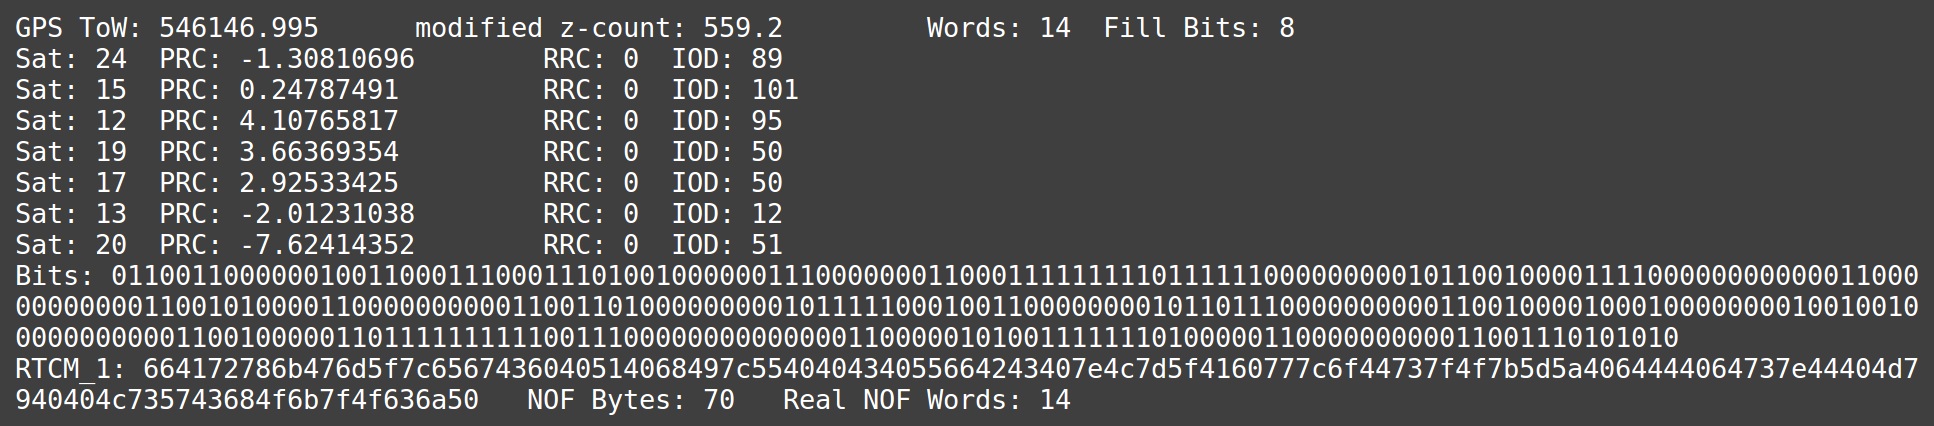
\includegraphics[width=\textwidth]{images/RTCM_Debug.png}
 \caption{Debug output for RTCM message 1}
 \label{fig:rtcm_debug}
\end{figure}
